% Options for packages loaded elsewhere
\PassOptionsToPackage{unicode}{hyperref}
\PassOptionsToPackage{hyphens}{url}
\PassOptionsToPackage{dvipsnames,svgnames,x11names}{xcolor}
%
\documentclass[
  letterpaper,
  DIV=11,
  numbers=noendperiod]{scrartcl}

\usepackage{amsmath,amssymb}
\usepackage{iftex}
\ifPDFTeX
  \usepackage[T1]{fontenc}
  \usepackage[utf8]{inputenc}
  \usepackage{textcomp} % provide euro and other symbols
\else % if luatex or xetex
  \usepackage{unicode-math}
  \defaultfontfeatures{Scale=MatchLowercase}
  \defaultfontfeatures[\rmfamily]{Ligatures=TeX,Scale=1}
\fi
\usepackage{lmodern}
\ifPDFTeX\else  
    % xetex/luatex font selection
\fi
% Use upquote if available, for straight quotes in verbatim environments
\IfFileExists{upquote.sty}{\usepackage{upquote}}{}
\IfFileExists{microtype.sty}{% use microtype if available
  \usepackage[]{microtype}
  \UseMicrotypeSet[protrusion]{basicmath} % disable protrusion for tt fonts
}{}
\makeatletter
\@ifundefined{KOMAClassName}{% if non-KOMA class
  \IfFileExists{parskip.sty}{%
    \usepackage{parskip}
  }{% else
    \setlength{\parindent}{0pt}
    \setlength{\parskip}{6pt plus 2pt minus 1pt}}
}{% if KOMA class
  \KOMAoptions{parskip=half}}
\makeatother
\usepackage{xcolor}
\setlength{\emergencystretch}{3em} % prevent overfull lines
\setcounter{secnumdepth}{-\maxdimen} % remove section numbering
% Make \paragraph and \subparagraph free-standing
\ifx\paragraph\undefined\else
  \let\oldparagraph\paragraph
  \renewcommand{\paragraph}[1]{\oldparagraph{#1}\mbox{}}
\fi
\ifx\subparagraph\undefined\else
  \let\oldsubparagraph\subparagraph
  \renewcommand{\subparagraph}[1]{\oldsubparagraph{#1}\mbox{}}
\fi

\usepackage{color}
\usepackage{fancyvrb}
\newcommand{\VerbBar}{|}
\newcommand{\VERB}{\Verb[commandchars=\\\{\}]}
\DefineVerbatimEnvironment{Highlighting}{Verbatim}{commandchars=\\\{\}}
% Add ',fontsize=\small' for more characters per line
\usepackage{framed}
\definecolor{shadecolor}{RGB}{241,243,245}
\newenvironment{Shaded}{\begin{snugshade}}{\end{snugshade}}
\newcommand{\AlertTok}[1]{\textcolor[rgb]{0.68,0.00,0.00}{#1}}
\newcommand{\AnnotationTok}[1]{\textcolor[rgb]{0.37,0.37,0.37}{#1}}
\newcommand{\AttributeTok}[1]{\textcolor[rgb]{0.40,0.45,0.13}{#1}}
\newcommand{\BaseNTok}[1]{\textcolor[rgb]{0.68,0.00,0.00}{#1}}
\newcommand{\BuiltInTok}[1]{\textcolor[rgb]{0.00,0.23,0.31}{#1}}
\newcommand{\CharTok}[1]{\textcolor[rgb]{0.13,0.47,0.30}{#1}}
\newcommand{\CommentTok}[1]{\textcolor[rgb]{0.37,0.37,0.37}{#1}}
\newcommand{\CommentVarTok}[1]{\textcolor[rgb]{0.37,0.37,0.37}{\textit{#1}}}
\newcommand{\ConstantTok}[1]{\textcolor[rgb]{0.56,0.35,0.01}{#1}}
\newcommand{\ControlFlowTok}[1]{\textcolor[rgb]{0.00,0.23,0.31}{\textbf{#1}}}
\newcommand{\DataTypeTok}[1]{\textcolor[rgb]{0.68,0.00,0.00}{#1}}
\newcommand{\DecValTok}[1]{\textcolor[rgb]{0.68,0.00,0.00}{#1}}
\newcommand{\DocumentationTok}[1]{\textcolor[rgb]{0.37,0.37,0.37}{\textit{#1}}}
\newcommand{\ErrorTok}[1]{\textcolor[rgb]{0.68,0.00,0.00}{#1}}
\newcommand{\ExtensionTok}[1]{\textcolor[rgb]{0.00,0.23,0.31}{#1}}
\newcommand{\FloatTok}[1]{\textcolor[rgb]{0.68,0.00,0.00}{#1}}
\newcommand{\FunctionTok}[1]{\textcolor[rgb]{0.28,0.35,0.67}{#1}}
\newcommand{\ImportTok}[1]{\textcolor[rgb]{0.00,0.46,0.62}{#1}}
\newcommand{\InformationTok}[1]{\textcolor[rgb]{0.37,0.37,0.37}{#1}}
\newcommand{\KeywordTok}[1]{\textcolor[rgb]{0.00,0.23,0.31}{\textbf{#1}}}
\newcommand{\NormalTok}[1]{\textcolor[rgb]{0.00,0.23,0.31}{#1}}
\newcommand{\OperatorTok}[1]{\textcolor[rgb]{0.37,0.37,0.37}{#1}}
\newcommand{\OtherTok}[1]{\textcolor[rgb]{0.00,0.23,0.31}{#1}}
\newcommand{\PreprocessorTok}[1]{\textcolor[rgb]{0.68,0.00,0.00}{#1}}
\newcommand{\RegionMarkerTok}[1]{\textcolor[rgb]{0.00,0.23,0.31}{#1}}
\newcommand{\SpecialCharTok}[1]{\textcolor[rgb]{0.37,0.37,0.37}{#1}}
\newcommand{\SpecialStringTok}[1]{\textcolor[rgb]{0.13,0.47,0.30}{#1}}
\newcommand{\StringTok}[1]{\textcolor[rgb]{0.13,0.47,0.30}{#1}}
\newcommand{\VariableTok}[1]{\textcolor[rgb]{0.07,0.07,0.07}{#1}}
\newcommand{\VerbatimStringTok}[1]{\textcolor[rgb]{0.13,0.47,0.30}{#1}}
\newcommand{\WarningTok}[1]{\textcolor[rgb]{0.37,0.37,0.37}{\textit{#1}}}

\providecommand{\tightlist}{%
  \setlength{\itemsep}{0pt}\setlength{\parskip}{0pt}}\usepackage{longtable,booktabs,array}
\usepackage{calc} % for calculating minipage widths
% Correct order of tables after \paragraph or \subparagraph
\usepackage{etoolbox}
\makeatletter
\patchcmd\longtable{\par}{\if@noskipsec\mbox{}\fi\par}{}{}
\makeatother
% Allow footnotes in longtable head/foot
\IfFileExists{footnotehyper.sty}{\usepackage{footnotehyper}}{\usepackage{footnote}}
\makesavenoteenv{longtable}
\usepackage{graphicx}
\makeatletter
\def\maxwidth{\ifdim\Gin@nat@width>\linewidth\linewidth\else\Gin@nat@width\fi}
\def\maxheight{\ifdim\Gin@nat@height>\textheight\textheight\else\Gin@nat@height\fi}
\makeatother
% Scale images if necessary, so that they will not overflow the page
% margins by default, and it is still possible to overwrite the defaults
% using explicit options in \includegraphics[width, height, ...]{}
\setkeys{Gin}{width=\maxwidth,height=\maxheight,keepaspectratio}
% Set default figure placement to htbp
\makeatletter
\def\fps@figure{htbp}
\makeatother

\KOMAoption{captions}{tableheading}
\usepackage{fontawesome5}
\makeatletter
\@ifpackageloaded{caption}{}{\usepackage{caption}}
\AtBeginDocument{%
\ifdefined\contentsname
  \renewcommand*\contentsname{Table of contents}
\else
  \newcommand\contentsname{Table of contents}
\fi
\ifdefined\listfigurename
  \renewcommand*\listfigurename{List of Figures}
\else
  \newcommand\listfigurename{List of Figures}
\fi
\ifdefined\listtablename
  \renewcommand*\listtablename{List of Tables}
\else
  \newcommand\listtablename{List of Tables}
\fi
\ifdefined\figurename
  \renewcommand*\figurename{Figure}
\else
  \newcommand\figurename{Figure}
\fi
\ifdefined\tablename
  \renewcommand*\tablename{Table}
\else
  \newcommand\tablename{Table}
\fi
}
\@ifpackageloaded{float}{}{\usepackage{float}}
\floatstyle{ruled}
\@ifundefined{c@chapter}{\newfloat{codelisting}{h}{lop}}{\newfloat{codelisting}{h}{lop}[chapter]}
\floatname{codelisting}{Listing}
\newcommand*\listoflistings{\listof{codelisting}{List of Listings}}
\makeatother
\makeatletter
\makeatother
\makeatletter
\@ifpackageloaded{caption}{}{\usepackage{caption}}
\@ifpackageloaded{subcaption}{}{\usepackage{subcaption}}
\makeatother
\ifLuaTeX
  \usepackage{selnolig}  % disable illegal ligatures
\fi
\usepackage{bookmark}

\IfFileExists{xurl.sty}{\usepackage{xurl}}{} % add URL line breaks if available
\urlstyle{same} % disable monospaced font for URLs
\hypersetup{
  pdftitle={In Praise of Documentation: Tools, Tips \& Techniques for Literate Programming in the AI Age},
  colorlinks=true,
  linkcolor={blue},
  filecolor={Maroon},
  citecolor={Blue},
  urlcolor={Blue},
  pdfcreator={LaTeX via pandoc}}

\title{In Praise of Documentation: Tools, Tips \& Techniques for
Literate Programming in the AI Age}
\author{}
\date{}

\begin{document}
\maketitle

\section{In Praise of Documentation}\label{in-praise-of-documentation}

\faBriefcase

This piece is in praise of documentation in data science and software
engineering. By the end of this talk, I hope to have convinced you that
documentation is a good thing, and that you should document your code.

I have one simple message: please document your code. Please. Document
your code.

I enjoy writing technical documentation. I enjoy trying to explain
things to people. Helping make sense of a report or a tool. But I
realise my enjoyment is not shared widely in the field.

While writing documentation is generally considered a ``good thing'',
many engineers in industry tend to either not document their work, or
document their work poorly.

I'll speculate about why this might be the case. And I'll argue why
better documentation is always a good thing. I'll give suggestions for
how you can write this documentation in the best way possible.

This piece is written as a \href{https://quarto.org/}{Quarto} document,
which is a Markdown format, that can be rendered into PDF or HTML
format. To illustrate how Quarto works, I'll ``show the code'',
reflexively illustrating how I wrote the documentation for this talk on
documentation.

\section{How I Learned to Love
Documentation}\label{how-i-learned-to-love-documentation}

I first discovered the pleasures of technical documentation 40 years
ago, as an 8 year old boy, using a BBC Microcomputer.

\begin{figure}[H]

{\centering 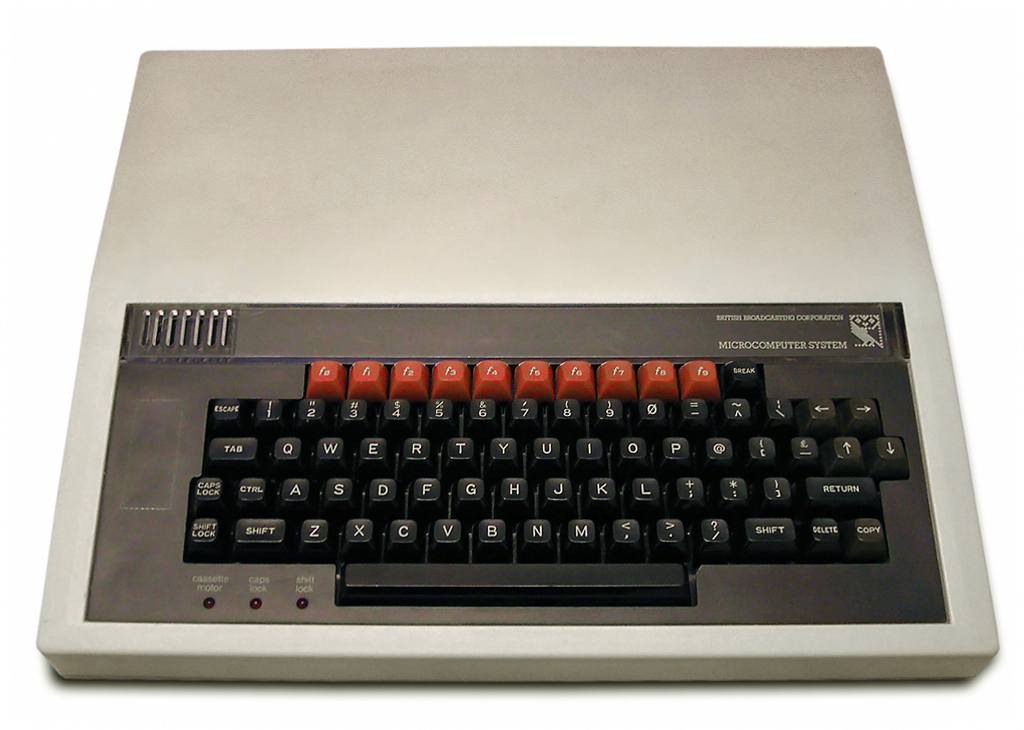
\includegraphics[width=0.8\textwidth,height=\textheight]{images/bbc_micro.jpg}

}

\caption{BBC Micro}

\end{figure}%

This computer was my best friend. The BBC Micro was an 8-bit computer,
funded by the British Broadcasting Corporation, and released in 1981 as
the centrepiece of their \href{https://clp.bbcrewind.co.uk/}{Computer
Literacy Project}.

This project aimed to make the British public more computer literate, by
making computers and programming more widely accessible to the massses,
mainly by making the BBC Micro available for use in schools
(\textbf{gazzard2016?}). The machine was designed and built by Acorn
Computers in Cambridge, England who also built my first computer, the
\href{https://en.wikipedia.org/wiki/Acorn_Electron}{Acorn Electron}, and
the \href{https://en.wikipedia.org/wiki/ARM_architecture_family}{ARM}
processor - now powering most mobile phones.

One of the distinctive features of the BBC Micro was that after you had
plugged the computer into your TV set, when you switched on the computer
(which made the sound ``beeee-beep''), you immediately found yourself on
what we now call a ``command line'', which looked something like this:

\begin{figure}[H]

{\centering \includegraphics[width=0.5\textwidth,height=\textheight]{images/bbc_basic.gif}

}

\caption{BBC BASIC}

\end{figure}%

I was faced with an immediate practical problem: how do I use this
thing? Remember, at the time, I have no mouse, and only a keyboard as my
input device, and there's no Graphical User Interface.

Thankfully, the computer came with a
\href{https://www.bbcmicrobot.com/docs/BBC_User_Guide.pdf}{User Guide}.

\begin{figure}[H]

{\centering 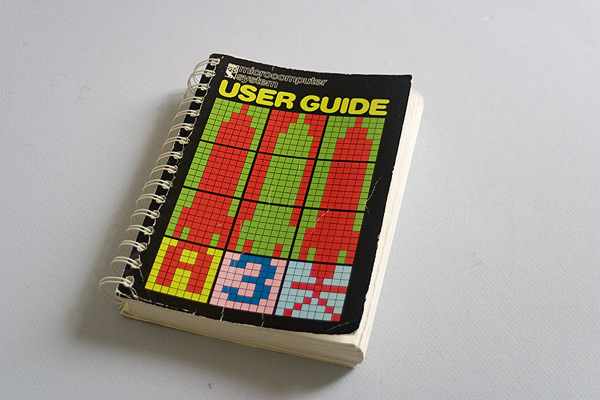
\includegraphics[width=0.5\textwidth,height=\textheight]{images/bbc_micro_user_guide.jpg}

}

\caption{User Guide}

\end{figure}%

It explained how to type BBC BASIC commands to ``run'' your programs
using the keyboard. The programs would run from cassette tapes or 5 1/4
inch diskettes. There was also a magazine,
\href{https://en.wikipedia.org/wiki/The_Micro_User}{BBC Micro User},
which I avidly collected.

\begin{figure}[H]

{\centering 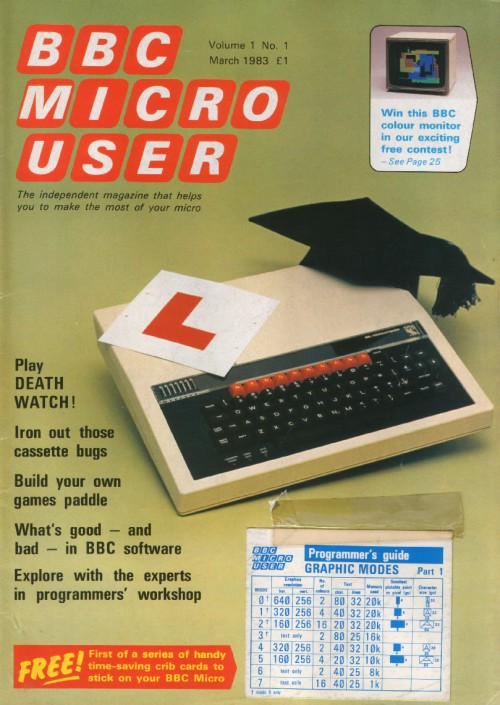
\includegraphics[width=0.5\textwidth,height=\textheight]{images/bbc_micro_user.jpg}

}

\caption{BBC Micro User}

\end{figure}%

I learnt to use the computer by reading this printed ``physical'' media.
To use the computer, I had to type commands. It turns out, these were
the commands of the programming language BBC BASIC. As soon as the
machine had booted up, and typing commands, I was already programming.
BBC BASIC was a scripting language, designed to be beginner-friendly, by
Sophie Wilson of Acorn Computers. I learnt to program in BBC BASIC by
manually typing out the `type-in program' code listings for computer
games in the magazines.

I tell you this story not only for nostalgic reasons, but also to
impress upon you the important role played by documentation in my early
experience with computers. Reading documentation was part-and-parcel of
learning to use the computer. And learning to program. I learnt early
the value of good documentation in democratising access to computers and
to understanding the code that the computers ``run'' on them. I also
learnt the value of early ``open source'' software in the form of
`type-in programs' in magazines.

In these early days of popular computing in Britain, learning the
technical task of computer programming was intimately tied to reading
the literature of documentation.

I later learned my early enjoyment for reading what we came to call
``docs'' was matched by an enjoyment in \emph{writing} technical
``docs''. I enjoyed trying to explain to people things that were
difficult to understand. Or describe how or why I did something the way
I did it. Or tell the story of some feature or analysis. Essentially, I
came to enjoy writing user guides.

I realised that by trying to explain something to someone, I often I
learnt something myself in the process. Something about what I had done.
Or what the analysis or the tool meant in the context of the project.
Even just trying to explain to someone \emph{how to run} some program
was often fascinating to me. I guess writing a user guide is offering
some kind of ``tech support''. Perhaps I felt I was being useful.

But I quickly realised other data scientists and software engineers
often didn't share my interest or indeed passion in ``docs''. I often
found people either wouldn't document their code at all, or they would
document it poorly, only under duress. This makes sense, in part, due to
the speed of work in industry. But I've found this attitude can lead to
not only poor practice, but can even have disastrous results in
companies.

\section{The Perils of Poor
Documentation}\label{the-perils-of-poor-documentation}

In one case, at a company to remain nameless, an entire data production
system - and I am using that phrase generously - along with the new
(second) cloud infrastructure built to replace it - were implemented
either without any documentation, or with very poor documentation.

The legacy system was filled with massive SQL scripts - a code version
of \emph{War and Peace} - with executed SQL code embedded into
configuration files (I never though this was possible), and with
production database login and password details hardcoded into a Python
script. All without any version control. (I never thought this was
possible either). And, just to add insult to injury, an entire Azure
Data Lake was implemented by a consultancy to fix the legacy system, in
addition to the existing cloud infrastructure, but was left without any
documentation at all.

It was not just the length of the SQL scripts that was the problem. The
SQL scripts themselves were not just long, they were convoluted, and
seemed to have been written in such a style as to make their meaning and
purpose entirely obscure to the reader.

I realise this is an extreme example. The ``bad'' things that can happen
without good documentation are probably usually more mundane. For
example, new colleagues might feel alienated in their team, or struggle
to learn a new and complex codebase, or be unable to easily update a
legacy system. It might take a whole team months, even years, to reverse
engineer a large codebase, in order to be in a position to rebuild or
replace it.

When digging into the archaeological sites of legacy codebases, I made a
more important realisation: code is a form of communication. Or, in many
cases, miscommunication.

How can we make our code communicate better? Or even communicate well?

\section{Why Document Your Code?}\label{why-document-your-code}

Before I answer this question about ``how'' to document our code, I'll
give evidence that it is not just me who thinks that documentation is a
``good thing''.

In her recent book \emph{Software Engineering for Data Scientists},
Catherine Nelson writes:

``Documentation is an often overlooked aspect of data science. It's
commonly left until the end of a project, but then you're excited to
move on to a new project, and the documentation is rushed or omitted
completely. However, \ldots{} documentation is a crucial part of making
your code reproducible. If you want other people to use your code, or if
you want to come back to your code in the future, it needs good
documentation. It's impossible to remember all your thoughts from when
you originally wrote the code or initially carried out the experiments,
so they need to be recorded.'' (\textbf{nelson2024?})

I would agree with all these points. I would also add that documentation
is essential for understanding the meaning of the code. Why does it do
what it does in the way that it does? Documentation is the best way to
answer this and similar questions.

\section{Types of Documentation}\label{types-of-documentation}

Nelson summarises different types of documentation that are relevant to
data science workflows. Here, I am directly quoting her recommendations:

\emph{Names}: Names of variables, functions, and files should be
informative, an appropriate length, and easy to read.

\emph{Comments}: Your comments should add extra information not
contained in the code, such as a summary or a caveat.

\emph{Docstrings}: Your functions should always have a docstring that
describes the inputs and outputs of the function, as well as the purpose
of that function.

\emph{READMEs}: Every repository or project should have an introduction
that advertises your code and lets other people know why they should use
it.

\emph{Jupyter notebooks}: Your notebooks will be much easier to read if
you give them good names, give them a structure, and intersperse text
and code.

\emph{Experiment tracking}: Experiments, especially in machine learning
projects, should be tracked in a structured way.

We can also think about technical documentation in terms of different
genres, which can help clarify the purpose of your documentation. The
\href{https://diataxis.fr/}{Diátaxis} is an interesting example. It
divides technical documents into four types:

\begin{itemize}
\item
  Tutorials
\item
  How-to guides
\item
  Technical reference
\item
  Explanation
\end{itemize}

When writing your documentation, you could think about the purpose of
the documentation, and which documentation type is most applicable for
your use case.

\section{Literate Programming}\label{literate-programming}

The advice given above by Nelson, especially the recommendation to use
Jupyter notebooks, can be considered advice for ``literate
programming''. Literate programming is perhaps the most commonly
recommended \emph{genre} or \emph{style} of computer programming for
data science. In literate programming, written prose is interspersed
with computer code, within the same document, called a ``notebook''. For
example, the following ``code cell'' executes a Python kernel (virtual
environment), which in turn executes the \texttt{print} function, and
the output of that function is displayed within the rendered document.

\begin{Shaded}
\begin{Highlighting}[]
\CommentTok{"""}
\CommentTok{This is a docstring. }
\CommentTok{It explains what a module, class, or function does.}
\CommentTok{Usually over multiple lines.}
\CommentTok{"""}
\CommentTok{\# This is a comment, an explanation, on a single line. I\textquotesingle{}m illustrating "classic" software documentation.}
\BuiltInTok{print}\NormalTok{(}\SpecialStringTok{f"How many fingers am I holding up, Winston? }\CharTok{\textbackslash{}n}\SpecialStringTok{ }\SpecialCharTok{\{}\DecValTok{2}\OperatorTok{+}\DecValTok{2}\SpecialCharTok{\}}\SpecialStringTok{"}\NormalTok{)}
\end{Highlighting}
\end{Shaded}

\begin{verbatim}
How many fingers am I holding up, Winston? 
 4
\end{verbatim}

Code execution can also be done in-line 4.

I was interested to find out when ``literate programming'' became
popuar, so I used Google Books Ngram Viewer search for this term from
1800 to 2026. This shows the frequency of use of this term in published
books.

\begin{Shaded}
\begin{Highlighting}[]
\NormalTok{\#| echo: false}

\NormalTok{curl {-}L "https://books.google.com/ngrams/json?content=\%22literate\%20programming\%22\&year\_start=1800\&year\_end=2026\&corpus=26\&smoothing=0" {-}o ngrams.json}
\end{Highlighting}
\end{Shaded}

I converted the JSON file to a CSV and then imported it as a DataFrame
using Polars.

\begin{verbatim}
DATA_DIR: ../data
\end{verbatim}

I use \href{https://pola.rs/}{Polars}, a DataFrame library written in
Rust, with an intuitive API, similar to
\href{https://dplyr.tidyverse.org/}{dplyr} in R.

You can render formatted tables from code. Here, I use the
\href{https://github.com/posit-dev/great-tables}{Great Tables} package,
based on the original \href{https://gt.rstudio.com/}{GT} package in R.
Great Tables has a cool ``nanoplot'' function, which allows you to
include a plot in a table.

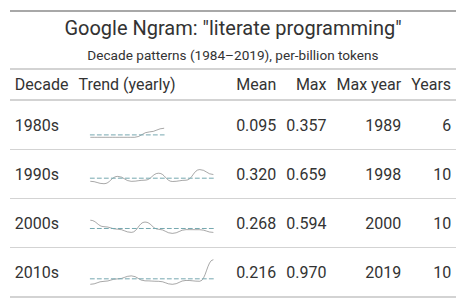
\includegraphics[width=0.8\textwidth,height=\textheight]{images/ngram_decade_summary.png}

You can also display plots. Here, I'm using
\href{https://plotnine.org/}{plotnine} which is a Python version of the
\href{https://ggplot2.tidyverse.org/}{ggplot2} data visualisation
library in R.

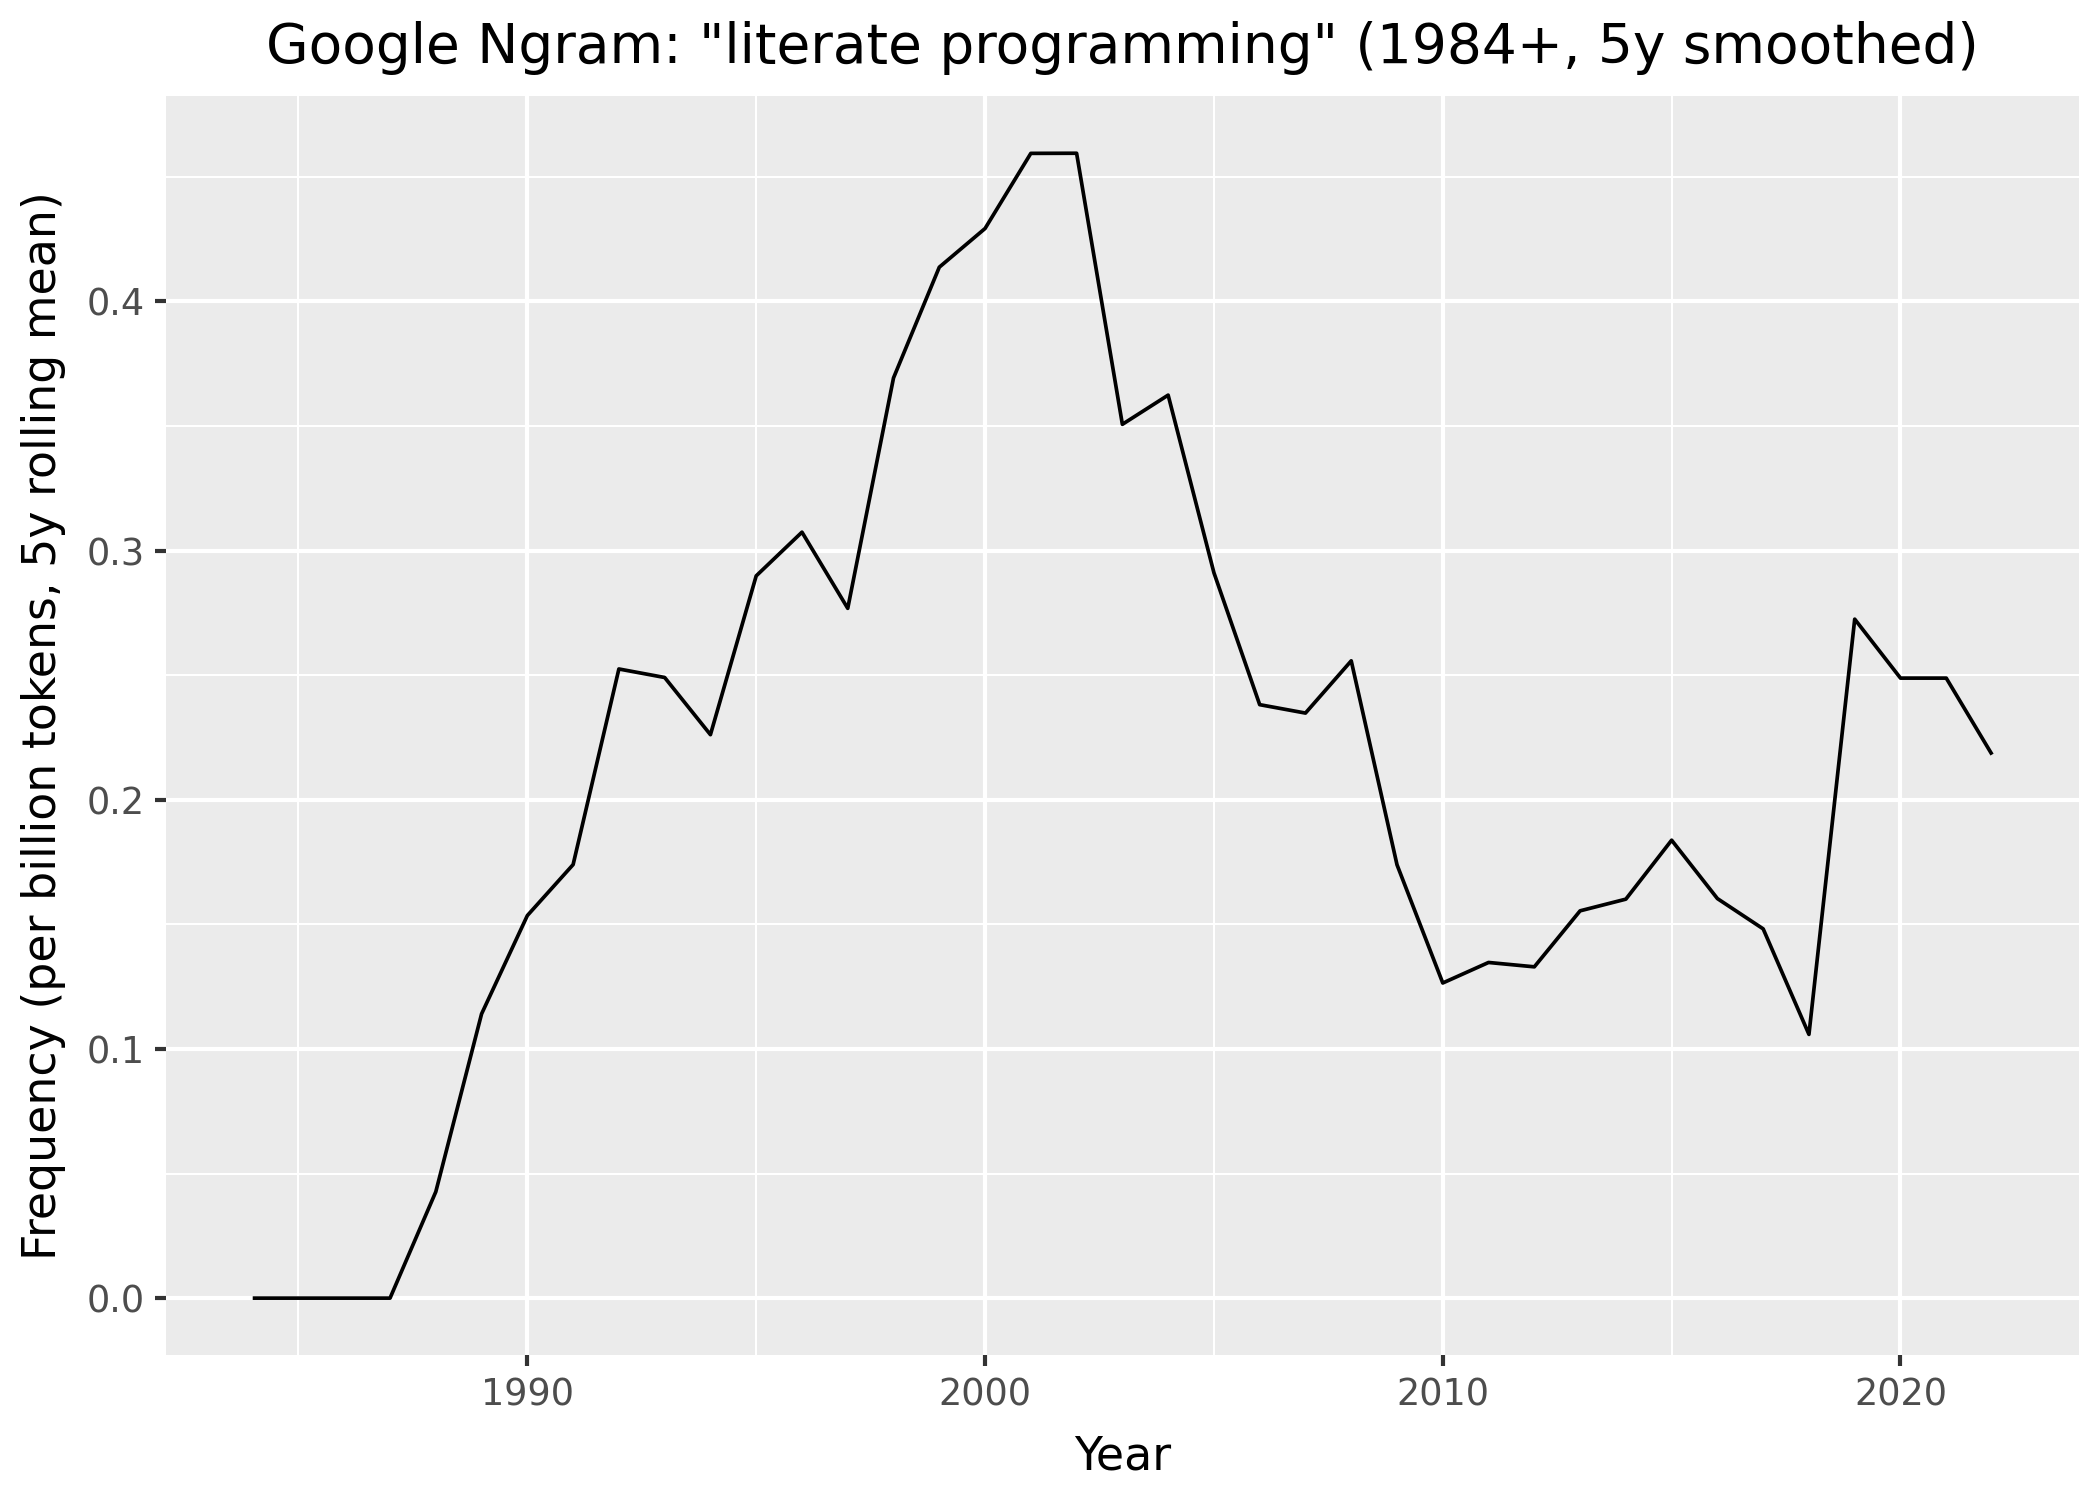
\includegraphics{images/ngram_literate_programming.png}

The popularity of the ``notebook'' format for data science makes sense,
because data science involves scientific programming, and the structure
advocated for literate programming resembles scientific writing -
especially the genre of the scientific laboratory report. This report
style is commonly structured into Introduction, Method, Results, and
Conclusion sections. The ``notebook'' allows the data scientist to use a
similar scientific report format. This is suitable for data exploration,
experimentation, and communicating the results of research - especially
reporting the findings of data analysis or machine learning experiments.
Notebooks can be run locally or in cloud environments like Azure
Synapse, Databricks, or Google Colab.

\section{History of Literate
Programming}\label{history-of-literate-programming}

While the basic technical implementation of literate programming will be
familiar to most data scientists, the origins and history of literate
programming might be less familar.

The term ``literate programming'' was coined in 1984, by the American
computer scientist Donald Knuth, later Professor Emeritus at Stanford
University (\textbf{knuth1984?}).

Knuth proposed literate programming as a new ``motto'' for software
development, building upon the foundations of ``structured
programming''. He built a system called \textbf{WEB} for implementing
this new genre of literate programming. Knuth suggests literate
programming is ``inherently bilingual'', because it combines two
different genres of writing within the same computer program files: a
document formatting language; a programming language. The document
formatting language is a typesetting system (TeX), which is used to
render an \emph{informal} English-language explanation of the program,
while the programming language (PASCAL) is the \emph{formal} computer
code, which is compiled by the compiler, and then executed by the user.

Knuth thereby developed a new literary form, reversing the traditional
``structured programming'' approach to documentation. In the
``structured programming'' approach, the formal computer code is
primary, and informal documentation is secondary, optionally embedded
into the code as \emph{comments}. We'll look at some examples of
comments later.

It is interesting to notice that Knuth's \textbf{WEB} system was
designed as a ``tool for systems programmers, not for high school
students or hobbyists'', because the programmer needs to be
``comfortable dealing with multiple languages simultaneously''
(\textbf{knuth1984?}).

40 years later, literate programming is most commonly adopted not by
systems programmers, but by data scientists who tend to use high-level
scripting languages (e.g.~R, Python, Julia). And the tools of literate
programming are considered particularly applicable for teaching and
learning programming (e.g.~Google Colab).

The preference for the notebook as a tool for literate programming in
education and data science might be due to the simplicitly of the
Markdown language that is used as the informal typesetting language
(rather than TeX). So the burdens on becoming ``bilingual'' might be
less than if they had to learn TeX.

\section{Scientific Publishing Tools}\label{scientific-publishing-tools}

Knuth's recommendations form the basis of contemporary technical tools
for later developments in scientific programming, later described as
data science, especially in the R and Python programming ecosystems.
These tools have been developed for cross-language programming
applications, especially for use in scripting languages (e.g.~R, Python,
and Julia). The technical implementation of literate programming is done
in a very similar way in the following scientific publishing tools:

\subsection{Jupyter and Marimo
notebooks}\label{jupyter-and-marimo-notebooks}

While Jupyter notebooks remain a key tool for data scientists in their
development work, they have a number of issues, which make them
difficult to scale up to production systems. As JSON files, they are not
straightforward to version control. Notebooks are designed so the cells
are run in their order of presentation, but cells can be executed out of
order, and then the notebook saved with outputs that do not match
execution order. And they can become quite large and unwiedly, leading
to IDE crashes, due to being bloated.

\subsection{R Markdown and Quarto}\label{r-markdown-and-quarto}

Explain \href{https://www.markdownguide.org/}{Markdown} and
\href{https://pandoc.org/}{Pandoc}.

\href{https://quarto.org/}{Quarto} is a scientific publishing system,
developed from the foundations of R Markdown. It uses text files with a
\texttt{.qmd} format. In short, you intersperse prose written in
Markdown format, with ``code cells'' which are enclosed with three
backticks for their start and end (`````).

At the top of the Quarto document is a YAML section, specifying the
configuration of the document:

\begin{verbatim}
---
title: "In Praise of Documentation: Tools, Tips & Techniques for Literate Programming in the AI Age"
format: 
    typst: 
        toc: false
bibliography: refs.yaml
bibliographystyle: apa
jupyter: pydata
---
\end{verbatim}

If you want to execute Python code cells in the document, Quarto uses
Jupyter to execute the Python via an iPyKernel virtual environment. In
this case, that environment is called \texttt{pydata}.

This Quarto document is configured to render as a PDF by default. To
render the document, on the command line, you type:

\begin{verbatim}
quarto render talk.qmd
\end{verbatim}

\section{Computer Programs as
Literature}\label{computer-programs-as-literature}

While Knuth's literate programming style has been widely implemented
into data science workflows, and will be familiar to most data
scientists, his original ideas about computer programming might be less
familar.

Knuth makes several arguments to support his ``motto'' of literate
programming:

\begin{quote}
``I believe that the time is ripe for significantly better documentation
of programs, and that we can best achieve this by considering programs
to be \emph{works of literature}''
\end{quote}

\begin{quote}
``Let us change our traditional attitude to the construction of progams.
Instead of imagining that our main task is to instruct a \emph{computer}
what to do, let us concentrate rather on explaining to \emph{human
beings} what we want a computer to do''.
\end{quote}

\begin{quote}
``The practitioner of literate programming can be regarded as an
essayist, whose main concern is with exposition and excellence of style.
Such an author, with thesaurus in hand, chooses the names of variables
carefully and explains what each variable means. He or she strives for a
program that is comprehensible because its concepts have been introduced
in an order that is best for human understanding, using a mixture of
formal and informal methods that reinforce each other''.
\end{quote}

This is a very unusual, and bold, set of arguments for a computer
scientist to make. I find it fascinating to think about now both data
science and software engineering more widely could be different, if
computer software was considered as works of literature.

If we were to seriously take on board what Knuth is saying, it seems to
me, the implications would go far beyond the creation of a new genre of
``literate programming'', which would come to be used mostly by data
scientists. I think the implications would reach far beyond scientific
computing and data science to the whole of software engineering.

I don't have time now to fully explore the implications of Knuth's
arguments. For now, I can say that, in the humanities, there is an area
called ``code studies'', which does treat computer code as literature,
and analyses that computer code as works of literature. But, as I
understand them, Knuth's arguments are to be applied primarily by
software developers, who tend to be engineers rather than artists or
poets or writers.

\section{Rules for Good Writing}\label{rules-for-good-writing}

To start small, we can follow in the spirit of Knuth, by taking
inspiration from once of the greatest writers of the 20th century.

In his 1945 essay \emph{Politics and the English Language}
(\textbf{orwell1945?}), George Orwell presented rules for how to write
well. While he was writing 80 years ago about the political language of
his time, his rules are relevant to writing technical documentation now.

Orwell called the use of language a habit. And he made a close
relationship between language and thought. By learning to write well, we
can develop good ways of thinking.

Orwell considered good writing to be active, precise, and simple. He
argued we should write actively rather than passively, be precise rather
than vague, and use simple verbs rather than complex longer words or
phrases. By writing clearly, we can think clearly, and thereby
communicate our thoughts more clearly to others. The thoughts are in the
words, and our thinking is displayed in our writing, so we had better
choose our words wisely.

Orwell's rules have particular relevance to writing in our dystopic age
of AI. Orwell was critical of lazy writing, where people use stock
phrases, rather than consciously choosing relevant words to express the
meaning of what is being written. Now, the risk is that we outsource our
thinking to AI, using Large Language Models to write our documentation
for us.

\section{Spec-Driven Development}\label{spec-driven-development}

\href{https://en.wikipedia.org/wiki/Spec-driven_development}{Spec-driven
development} reverses the usual approach to documentation in software
engineering, where documentation is written \emph{after} the software
itself. Instead, specifications are written in a machine-readable
format, which can then be read by coding agents.

\begin{itemize}
\item
  \href{https://agents.md/}{AGENTS.MD} is an emerging standard way of
  implementing spec-driven development. \texttt{AGENTS.md} is text file
  in Markdown format, written to be read by coding agents, which they
  use to create a plan and then execute that plan.
\item
  Example coding agent tools which can read this file include the Cursor
  IDE, OpenAI Codex, and Claude Code.
\end{itemize}

I've included an example \texttt{AGENTS.md} file in the root of the
repository.

\section{Conclusion}\label{conclusion}

When building data systems, or doing data analysis, we are \emph{writing
text}. When we code, we are writing. And, if we write technical
documentation, we are also writing.

When we write, we should should write with a reader in mind. Like a
presentation has an audience, a written document has a reader. This
reader might be our future self. Or a colleague who needs to learn about
some report or tool. Or even an AI agent we are instructing.

The code we write now will be read by our future selves, future users of
our software, and future readers of our reports, or users of our
software tools.

In writing our code today, we are writing the legacy code of tomorrow.

In this sense, coding is a mode of communication.

Documentation is a user guide for the legacy code infrastructures of the
future.

Writing good documentation can help you feel good, and make the world a
better place.

Writing good documentation allows us to:

\begin{itemize}
\item
  Preserve institutional and personal memory
\item
  Ensure scientific reproducibility
\item
  Allow better version control so that our software is robust
\item
  Enable responsible stewardship of technical systems through
  maintenance
\end{itemize}

\section{Resources}\label{resources}

\href{https://www.writethedocs.org/guide/}{Write the Docs}: best
practices for creating software documentation and technical writing.

Ghost: ``Revisioning data science in the age of AI''



\end{document}
